%% ============================================================
%% Chapter 3 — Results
%% ============================================================
\chapter{Results}\label{chapter:3_Results}
This chapter should present the results obtained during the preparation of the thesis. They should constitute a logical extension of the theoretical part and the design methodology. The description should include the obtained outcomes. It is also necessary to explain what they mean, i.e., provide their interpretation. The description should evaluate the results, indicating their significance and reliability. It is also advisable to compare them with other solutions, theoretical data, or expected outcomes. Depending on the kind of thesis, this chapter may also include a detailed list of the methods, tools, or technologies used, along with examples of their practical applications.

\section{Illustrative elements and results analysis}
\noindent This subsection presents example ways of displaying results, including:
\begin{itemize}
  \item mathematical formulas (with numbering on the right-hand side of the column),
  \item figures (with captions placed under the illustration, continuous numbering),
  \item tables (with the title above the table and units in a separate column),
  \item as well as the rules for referring to these elements in the text.
\end{itemize}

\noindent Using the command \verb|\noindent|, it is possible to continue a paragraph (without indentation).

%% ------------------------ Formulas --------------------------
\subsection{Editing formulas}
Mathematical formulas should be inserted using the \verb|equation| environment, which automatically assigns numbering, e.g.:
\begin{equation}
\label{eq:linear_equation}
\mathbf{A}x=b,
\end{equation}
\noindent where:

\vspace*{0.5em}
\begin{tabular}{@{}lll}
$\mathbf{A} \in \mathbb{R}^{n\times n}$ &-&coefficient matrix,\\
$\mathbf{x} \in \mathbb{R}^{n}$         &-&vector of unknowns,\\
$\mathbf{b} \in \mathbb{R}^{n}$         &-&right-hand-side vector.
\end{tabular}
\vspace*{0.5em}

\noindent Each formula should be referenced in the text using the command \verb|\eqref{}|, as shown in equation \eqref{eq:linear_equation}. All symbols used in the formula should be unambiguously explained directly below it. Variables and physical quantities should be written in italics, e.g., $x$, whereas matrices and vectors should be in bold mathematical font, e.g., $\mathbf{A}$. One should also remember the rules for writing numerical values (no space before the minus sign), e.g., $-$20, and separating units with a space, e.g., 5 V, or using the command \verb|\:| inside a mathematical operator, e.g., 10$\:  \frac{\mathrm{m}}{\mathrm{s^2}}$. If possible, equations should not be inserted directly in the paragraph. If a system of equations needs to be presented, the \verb|cases| environment may be used:
\begin{equation}
\begin{cases}
x + y = 5,\\
2x - y = 1.
\end{cases}
\label{eq:uklad}
\end{equation}
\enlargethispage{\baselineskip}
%% ------------------- Plots and graphics ---------------------
\subsection{Plots and graphics}
Each plot or figure should have a number and a caption placed below the illustration. Please note here that the font size (Arial 9 pt), axis proportions, and overall aesthetics of the plot should be preserved. size (Arial 9 pt), axis proportions and the overall aesthetics of the plot. Vector formats are recommended (e.g., .eps, .pdf, .svg), as they preserve full quality when scaling. Raster graphics (e.g., .png, .jpg) from low-resolution screenshots should be avoided. A figure should be inserted using the \verb|figure| environment with the \verb|[!htbp]| option to keep its position in a given place in the text, e.g.:

\begin{figure}[!htbp]
  \centering
  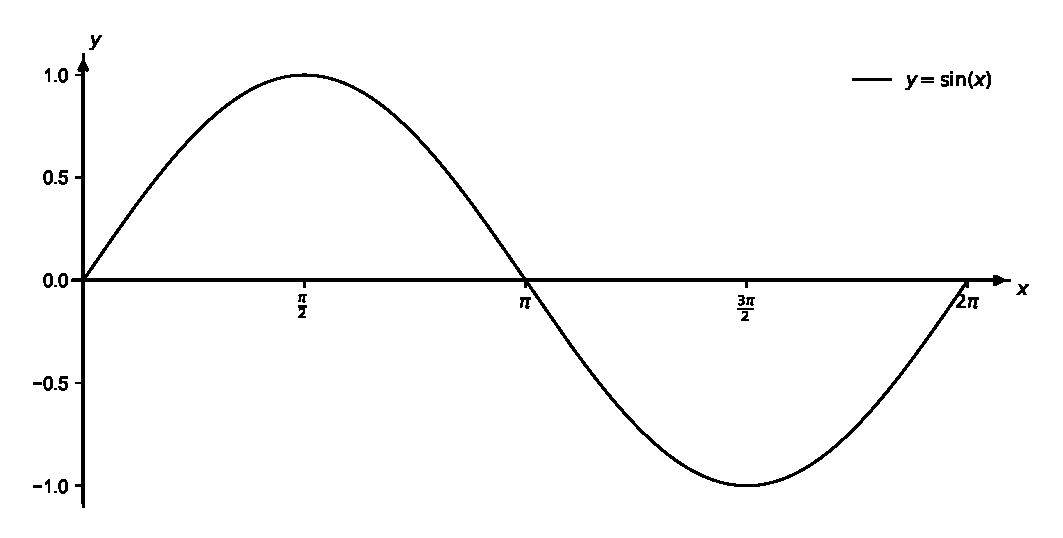
\includegraphics[width=1\linewidth]{img/sin.eps}
  \caption{Plot of the sine function. The Python program code of the plot is provided in Appendix \ref{page:A_appendix}.}
  \label{fig:sin}
\end{figure}

\noindent LaTeX automatically generates the list of figures after using the command \verb|\listoffigures|. When using external materials (e.g., photos, plots, diagrams), the source must be indicated and care taken not to infringe copyright.

%% --------------------------- Tables -------------------------
\subsection{Tables}
In an engineering thesis, it is useful to use tables (placed in the \verb|table| environment) to present sets of technical parameters, measurement results, system configurations, or performance comparisons. The title is placed above the table (command \verb|label|). If the table is extensive, it can be used the command \verb|\resizebox{\textwidth}{!}{...}| or the \verb|longtable| package for tables spanning multiple pages. Remember to refer to the table in the text using the command \verb|\ref{}|.

\begin{table}[!htbp]
\centering
\caption{Summary of the basic parameters of the test system}
\label{tab:test_params}
%% @{} -> removes the inner padding at the left/right table edges
%% \raggedright -> aligns left
%% p{.28\linewidth} -> column of fixed width: 28% of the table width
%% X fills the remaining width; wraps lines like p{...}
%% >{\centering\arraybackslash}p{.13\linewidth} -> fixed-width 13% column, centered;
%% \arraybackslash restores default behaviour at the end of the cell
\begin{tabularx}{\linewidth}{@{}>{\raggedright\arraybackslash}p{.28\linewidth}>{\raggedright\arraybackslash}X
                              >{\centering\arraybackslash}p{.13\linewidth}
                              >{\centering\arraybackslash}p{.13\linewidth}@{}}
\textbf{Parameter} & \textbf{Description} & \textbf{Value} & \textbf{Unit} \\ \hline
Clock frequency & Main clock frequency of the microcontroller & 80 & MHz \\
Supply voltage & Value of the input voltage & 5.0 & V \\
Current consumption & Average current consumption during operation & 120 & mA \\
Operating temperature & Safe operating range of the device & $-$10 – 60 & °C \\
Sampling time & Measurement interval in the main loop & 50 & ms \\
Number of input channels & Number of supported analogue sensors & 8 & – \\
Type of data transmission & Communication protocol used for transmission & UART & –
\end{tabularx}
\end{table}
\FloatBarrier


%% ----------------- Chapter summary --------------------------
\section{Chapter summary}
The results chapter should end with a summary of the most important observations and conclusions drawn from the analysis. It is also worth noting the investigation's potential limitations and areas requiring further testing and comparison.
